\subsection{Magnetic force between magnet and coil}

\begin{samepage}
    To calculate the magnetic repulsion force between the coil and a permanent magnet we consider them aligned with their centers coinciding on the z-axis.
    \nopagebreak

    \begin{figure}[H]
        \centering
        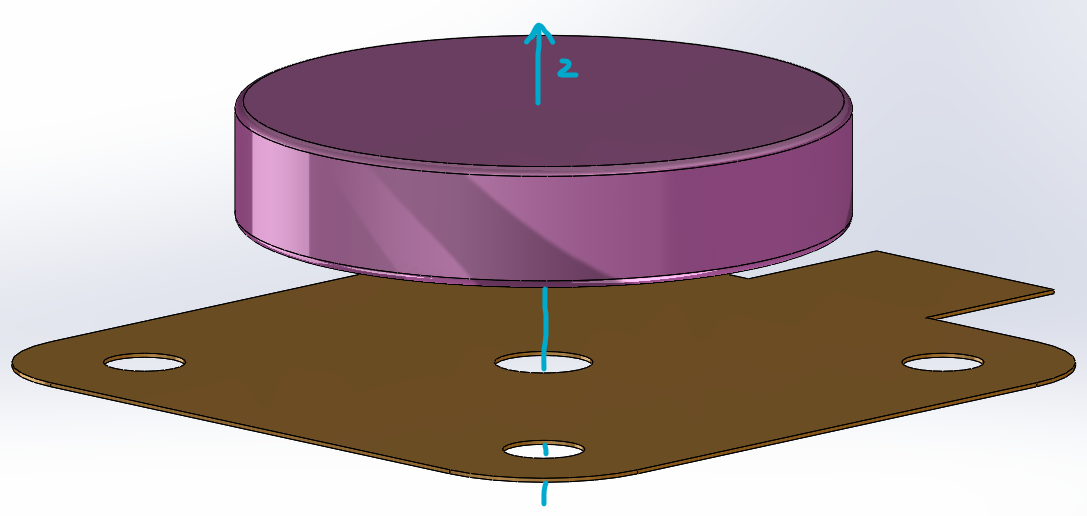
\includegraphics[width=0.5\columnwidth]{Chapters/Chapter2/Modelling_of_Entire_System/Figures/coil_magnet.png} 
        \caption[Coil-Magnet position]{Coil and magnet position in space.}
        \label{fig: Coil-Magnet_position}
    \end{figure}
\end{samepage}

\begin{samepage}
    The force between a magnet and a coil can be calculated using the magnetic field generated by the two.
    Knowing their closed-form expression we can calculate the force using the equation for magnetic levitation between a permanent magnet and planar magnetic serpentines \cite{wiki:magnetic_levitation}.
    \nopagebreak

    \begin{equation}
        F = \nabla (\overrightarrow{m_M} \cdot \overrightarrow{B_C}) % TODO: trovare fonte migliore di https://en.wikipedia.org/wiki/Magnetic_levitation
        \label{eq: Magnetic_force_coil_magnet}
    \end{equation}
    \nopagebreak

    Where: 
    \begin{itemize}
        \item $\overrightarrow{m_M}$ is the magnetic moment of the magnet [A/m]
        \item $\overrightarrow{B_C}$ is the magnetic field generated by the coil [T]
    \end{itemize}
\end{samepage}

\begin{samepage}
    The magnetic momentum of the magnet is defined as:
    \begin{equation*}
        \overrightarrow{m_M} = 
        \begin{pmatrix}
            0 & 0 & \frac{B_M(z)}{\mu}
        \end{pmatrix}
    \end{equation*}
    \nopagebreak

    Where:
    \begin{itemize}
        \item $B_M(z)$ is the magnetic field generated by the permanent magnet [T]
        \item $\mu$ is the magnetic permeability of the medium [H/m]
    \end{itemize}
\end{samepage}

We can calculate the magnetic field generated by the coil at a distance using equation \ref{eq: Spiral_magn_field_dist} (considering our coil as two in series) and the magnetic field generated by a cylindrical magnet at a distance $z$ using equation \ref{eq: Magnetic_field_perm_magnet}.

\begin{samepage}
    Doing the calculations, the resulting force in function of the distance $z$ is given by:
    \nopagebreak

    \begin{equation*}
        F = \frac{ B_r I N R_C^2 \left(\frac{1}{\sqrt{\sigma_1}} - \frac{1}{\sqrt{\sigma_2}} + \frac{z^2}{\sigma_2^{3/2}} - \frac{2(t+z)^2}{2\sigma_1^{3/2}}\right)}{2\sigma_3^{3/2}} + B_C(I) \cdot \frac{3z \left(\frac{z}{\sqrt{\sigma_2}} - \frac{t+z}{\sqrt{\sigma_1}}\right)}{2\sigma_3}
    \end{equation*}
    \nopagebreak

    Where:
    \nopagebreak

    \begin{itemize}
        \item $N$ is the number of spires of a one-layer coil
        \item $I$ is the current flowing through the coil [A]
        \item $B_C$ is the coil magnetic field calculated as in \ref{eq: Spiral_magn_field_dist} [T]
        \item $R_C$ is the coil average radius ($r'$ in equation \ref{eq: Spiral_magn_field_dist}) [m]
        \item $\sigma_1 = R_M^2 + (t+z)^2$
        \item $\sigma_2 = R_M^2 + z^2$
        \item $\sigma_3 = R_C^2 + z^2$    
    \end{itemize}
\end{samepage}

\pagebreak

\begin{samepage}
    So we can model the coil-magnet system as a \textbf{transducer} element that converts the current flowing through the coil into a force acting on the magnet.
    \nopagebreak

    \begin{equation*}
        B_C(z, I) = \frac{\mu N I R_C^2}{2(R_C^2+z^2)^\frac{3}{2}} \rightarrow B_C(q, i) = \frac{1}{2} L(q) i
    \end{equation*}
    \nopagebreak

    \begin{figure}[H]
        \centering
        \resizebox{.7\linewidth}{!}{
            \begin{tikzpicture}
    \begin{scope}[every node/.style={bgelement}]
    \node (start) at (0,0) {};
    \node[right=1 of start] (CI) {CI: Coil+Magnet};
    \node[right=1 of CI] (end) {};
    \end{scope}
    \draw[bonds]
    (start) edge [e_in, flow={i}, effort={V}] (CI)
    (end) edge [e_in, flow={v}, effort={F}] (CI);
\end{tikzpicture}
    
        }
        
        \begin{equation*}
            F(q, i) = \frac{1}{2} \frac{d \left(L(q) \cdot m_M(q) \right)}{dq} i
        \end{equation*} 
        \begin{equation*}
            \lambda = L(q) i
        \end{equation*}
        \caption{Coil-Magnet Transducer bond graph.}    
        \label{fig: Coil-Magnet_Transducer}
    \end{figure}
\end{samepage}

The last two equations represent the \textbf{standard notation for the constitutive equations} of the transducer element we described.
The equation for the force (derived from \ref{eq: Magnetic_force_coil_magnet}) represents the relation between the \textbf{input flow} (the coil current $i$) and the \textbf{output effort} (the force $F$).
Meanwhile, \textbf{$\lambda$} represents the \textbf{flux of the coil} which in this case is the \textbf{output flow} of the transducer.